\chapter{Introduction}

Psychological resilience is generally regarded as positive adaptation to past and ongoing exposure to potential negative effects of stressors. Accordingly, adaptation to stressful or adverse situation is a dynamic process with predictors that can differ between population groups. Within the discipline of developmental psychology, Tuescher and colleagues have provided prospective studies investigating the concept of resilience and its complex underlying mechanisms. As part of a doctoral dissertation, their studies aimed to validate the following research questions:

\begin{itemize}
    \item Does resilience have a positive effect on the willingness to participate in politics, specifically in election?
    \item Does the confrontation with positive or negative statements on politics for people with lower resilience have stronger effects on the willingness to participate in politics?
\end{itemize}

The research group did its poll by selecting people from Mainz, while trying to generalize to the entire German population. The survey data (GBS, n=587) tends to over-represent groups of higher income and higher education, since participants are primarily selected from an academic environment.

Therefore, the validity of assertions about the population beyond the original observation range is affected, even if statements are made conditional upon the available data. The basic premise for standard statistical conclusions, that the training and test set are drawn independently and identically (i.i.d.) from the same probability distribution, does not hold any more. This setting is also known as covariate-shift (Shimodaira 2000). Data sets are rarely generated under ideal conditions with bias pervasive in almost all empirical studies. The oftentimes underestimated analytic errors produce misleading descriptions of populations and ultimately yield false inferences (Aurelien, West, Sakshaug, 2016).

To get a complete picture of the subject, the research group consulted the department Data Archives for the Social Sciences. Their data archive service (GESIS) holds representative data of comparable studies in politics and psychology. The acquired sample (GESIS, n=4000) encompasses the German speaking population with permanent residence in Germany. 

This thesis is a practical application to reduce the sampling bias by selecting a maximal representative subsample (MRS) of GBS survey respondents with reference probability distributions from GESIS. The effects of positive and negative treatments on political participation are then analysed in the resulting MRS and compared to the initial GBS data [Fig. 1.1].

To evaluate the research questions to a certain required level of significance, it is inevitable to keep the exclusion of instances at a minimum. Pruning the GBS data in any way, narrows the data variance and thus the reach of subsequent studies. This is especially harmful since the initial GBS survey data is already small.

\vspace{20pt}
\begin{figure}[ht]
	\begin{center}
		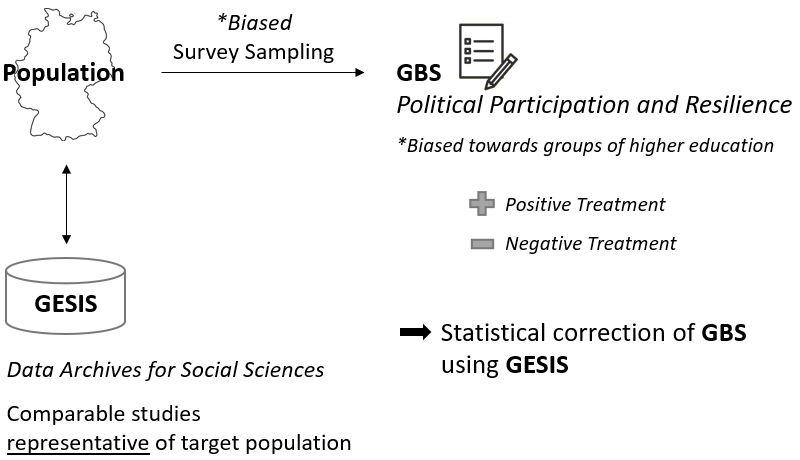
\includegraphics[scale=0.60,angle=0]{fig/overview}
		\label{project}
		\caption{Multivariate auxiliary information GESIS linked to GBS so that expected bias can be detected and corrected for. In addition, GBS contains an attribute for positive or negative treatment of survey participants for further analysis.}
	\end{center}
\end{figure}

In the MRS procedure, discriminative learners will look for decision boundaries to distinguish the negative class GBS from the positive class GESIS. First, both data sets are combined by adding an attribute indicating the source of origin. This label is predicted so that instances can be ranked according to their predicted probability. GBS participants that can be distinguished are removed from the result set. The remaining instances in GBS define the MRS and are expected to be more closely aligned with the target probability distribution.  The area under the receiver operating characteristic curve (AUROC) is used as single number evaluation metric to measure the degree of sampling bias. The MRS is characterized by an AUROC of roughly 0.5.

The fraction of misclassified GBS instances is kept as proxy measure for the subsequent method positive-unlabeled learning (Denis et al. 2005). Positive-unlabeled learning is a semi-supervised technique that does not make the simplifying assumption of GBS being positive or negative. GBS is in actual fact unlabeled, i.e. subgroups of the target population might be over-represented or actually representative. Apparently, subsampling does not help in the case of under-represented subgroups.

These procedures can only work when most of the observations come from a feature space which is not specific to one of the surveys. Thus, attributes must be matched correctly. 

\section{Related Work}

The influence of sampling bias could be alleviated by weighting the instances according to their importance (Shimodaira 2000). Statistical adjustment might also be reached by developing survey weights for calibration estimators [5]. However, these techniques require density estimation which is known to be a hard problem especially in high-dimensional cases (Haerdle et al. 2004). Directly estimating the importance without estimating the density ratios would be more promising: Discriminative machine learning for maximal representative subsampling.

\section{Outline}

The remainder of this thesis is organized as follows. Sec. 2 starts with an initial data analysis step and focuses more narrowly on checking assumptions required for model fitting and hypothesis testing, i.e. handling missing values and making transformations of variables. Sec. 3 defines key terminology and definitions and discusses discriminative learning and positive-unlabeled learning. The resulting maximal representative subset of GBS is presented in Sec. 4 and compared to GBS regarding political participation and resilience. Sec. 5 concludes.
